Um die Entwicklung für die Codebasis so einfach wie möglich zu machen wurde Git verwendet. Es handelt sich um ein Versionskontrollsystem, das hauptsächlich von Entwicklern zur Verwaltung der verschiedenen Versionen ihres Codes verwendet wird. Das Ziel hinter Git steckt darin die Entwicklung für ein Team von mehrern Entwicklern so einfach wie möglich zu gestalten. Im April 2005 begann der Entwickler des Betriebssystems Linux Linus Torvalds mit der Entwicklung von Git und präsentierte bereits wenige Tage nach der Ankündigung die erste Version der Code Verwaltungs Software.

\cite{Git}

\subsubsection{Repository}

Ein Git-Repository ist ein Speicherort, in dem Git, ein weit verbreitetes Versionskontrollsystem, Dateien und Verzeichnisse speichert. Bereits ein normaler Ordner kann ein Repository werden. Hierzu muss nur ein spezieller Befehl im Terminal ausgeführt werden, dieser erstellt einen .git Ordner in welchem die verschiedenen Versionen der Dateien gespeichert werden. Wichtig zu wissen ist auch das die Dateien im .git Ordner nicht manuell geändert werden sollten, da dies zu Problemen führen könnte.

\subsubsection{Commit}

Um eine neue Version von einer oder mehreren Dateien zu speichern muss ein Commit gemacht werden. Bevor ein Commit gemacht wird müssen die einzelnen Änderungen in den sogenannten "Staging-Bereich" hinzugefügt werden. Es können entweder spezifische Dateien hinzugefügt werden oder alle Dateien welche Änderungen beinhalten. Zum Beispiel :

\begin{verbatim}
git add <dateiname>.txt # Eine bestimmte Datei hinzufügen
git add . # Alle geänderten Dateien hinzufügen
\end{verbatim}

\subsubsection{Branches}

Branches werden in größeren Entwickler Teams meistens für einzelne Features verwendet. Somit wird sichergestellt, dass die einzelnen Teammitglieder nicht versehentlich Änderungen in einer Datei vornehmen die für ein anderes Feature essenziell sind. Beim erstellen von einem Branch wird im Hintergrund an und für sich nur eine Kopie des main Branches erstellt. Der Branch kann mit dem Befehl: 

\begin{verbatim}
    git checkout <branchname>
\end{verbatim}

gewechselt werden.
In einem Branch kann der Entwickler quasi frei arbeiten ohne die Arbeit eines Teammitglieds zu bearbeiten, solange er seinen Branch nicht in einen anderen merged.

<image>

\cite{Github_Branches}

\subsubsection{Merge}

Mit dem Merge Befehl werden einer oder mehrere Zweige (Branches) zusammengeführt. Dies ist in Git eine sehr häufige Operation welche verwendet wird um den Code aus einem Quellzweig in den Zielzweig zu bringen.
Ein Merge wird mit folgendem Befehl ausgeführt: 

\begin{verbatim}
    git merge <branchname>
\end{verbatim}

Hierbei kann es zu Konflikten kommen. Dies geschieht normalerweise, wenn zwei oder mehr Zweige gleichzeitig Änderungen an derselben Stelle in einer Datei oder an einer Datei vornehmen. Git kann hier nicht automatisch entscheiden welche Version es behalten soll und so muss der User manuell entsheiden welche Version verwertet und welche verworfen werden soll. Mit dieser Funktion können Änderungen von Zweigen sehr einfach in den Main Branch gebracht werden.

\begin{figure}[h!]
    \centering
    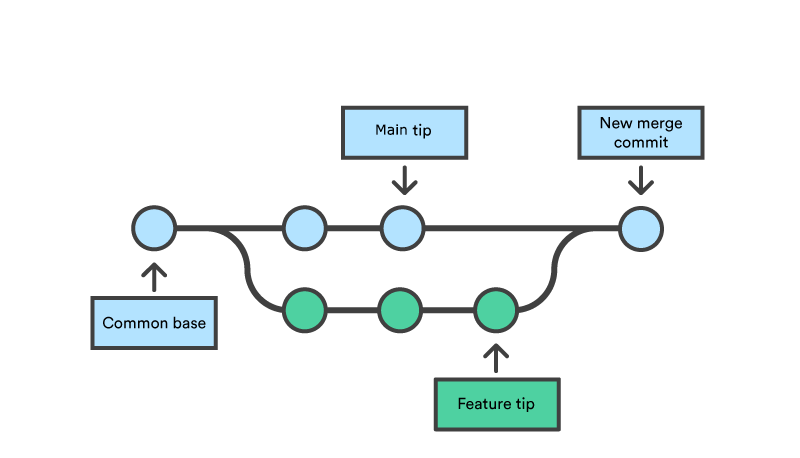
\includegraphics[width=0.6\linewidth]{pics/merge.png}
    \caption{Wie funktioniert ein Merge}
    \label{fig:enter-label}
\end{figure}

\subsection{Git cloud solutions}

Um als Team mit Git zu arbeiten ist es wichtig, dass alle Änderungen zwischen den Usern und den verschiedenen Geräten synchronisiert werden. Hierfür werden Git cloud solutions verwendet. Eine der bekanntesten ist Github, diese Plattform wird von den meisten Entwicklern verwendet.

\subsubsection{Github}

Github ist einer der Gründe wieso Git so berühmt wurde. Es wurde 2008 gelaunched und war damals eine der ersten git hosting Plattformen welche die Zusammenarbeit zwischen mehreren Entwicklerun um einiges vereinfachte. Github bietet sehr viele kostenlose Features an solange das Repository öffenltich ist. Um ein privates Repository zu besitzen und diese Features trotzdem verwenden zu können ist ein Abonnoment nötig.

\cite{Github_1}
\cite{Github_2}